\documentclass[letterpaper, 12pt]{math}

\usepackage{graphicx}
\usepackage{listings}
\lstset{basicstyle=\ttfamily\footnotesize,breaklines=true}
\geometry{letterpaper, margin=0.8in}

\title{CSCI 251: Concepts of Parallel and Distributed Systems}
\author{Alvin Lin}
\date{September 2017 - December 2017}

\begin{document}

\maketitle

\section*{Project 1}
This project involved the implementation of the Gauss-Jordan elimination
algorithm to reduce an augmented matrix to reduced row echelon form. This
implementation was done in C serially, and the parallelized using POSIX threads.
The serial implementation of the algorithm involved iterating through each
row of the matrix and reducing all the columns in the other rows to zero via
the elementary row operations. To parallelize this operation, the rows were
simply distributed among the threads for computation.

\subsection*{Serial Psuedocode}
This implementation assumed that the given augmented matrix was consistent
and that the coefficient matrix was \( n\times n \). Thus the augmented matrix
is of dimension \( n\times (n+1) \).
\begin{lstlisting}
def solve(matrix):
    let n = rows of matrix
    for i = 0 to n:
        for j = 0 to n:
            if i != j:
                let c = matrix[j][i] / matrix[i][i] # scaling factor
                for k = 0 to n + 1:
                    matrix[j][k] -= c * matrix[i][k]
    for i = 0 to n:
        matrix[i][n] /= matrix[i][i]
        matrix[i][i] = 1
    return matrix
\end{lstlisting}

\subsubsection*{Analysis}
The full data sheet of the runtimes is in the included data.pdf file.
In terms of the runtimes, as data size increased, runtimes improved the more
threads we used.
\begin{center}
  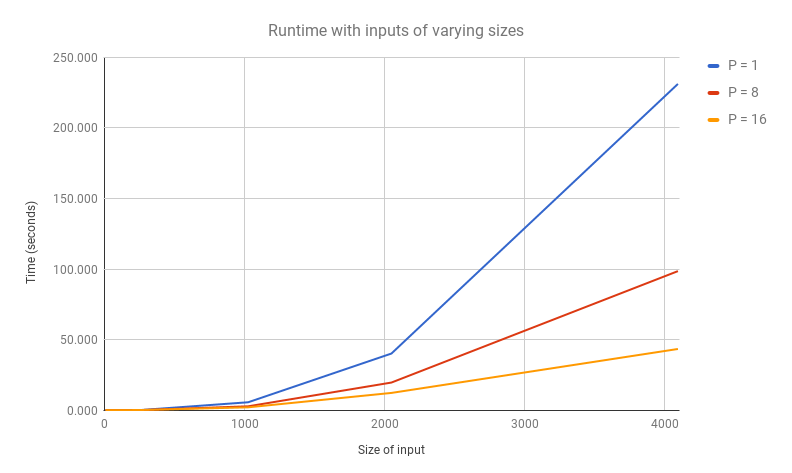
\includegraphics[width=16cm]{assets/runtime.png}
\end{center}
At low data sizes though, the extra threads caused overhead and led to a
decrease in speedup. In general however, more threads allowed for better
performance at high input sizes.
\begin{center}
  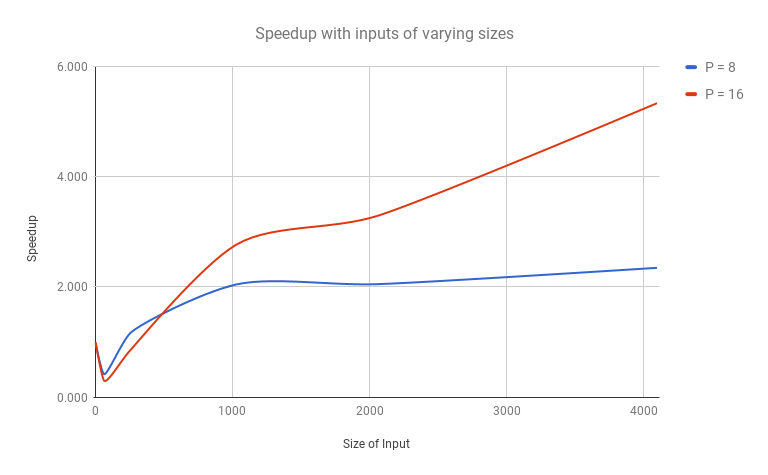
\includegraphics[width=16cm]{assets/speedup.png}
\end{center}


\end{document}
